%!TEX root = ../report.tex

\section{Architectural Patterns}

\subsection{Layer Pattern}
Structure:\\
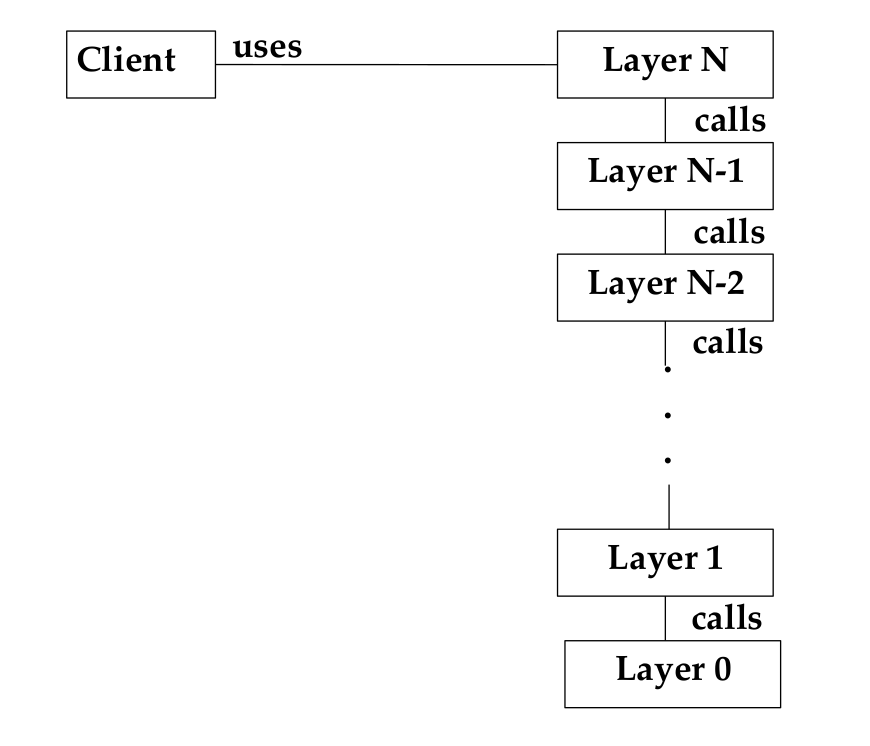
\includegraphics[width=.75\linewidth]{images/pattern_layer.png}
\begin{description}
  \item[Closed Architecture (Opaque Layering):]\hfill \\
    Each layer can only call operations from the layer below.\\
  \item[Open Architecture (Transparent Layering):]\hfill \\
    Each layer can call operations from \textbf{any} layer below
\end{description}

\textbf{5 Steps to Create a Layered Architecture}
\begin{enumerate}
  \item Identify subsystems
  \item Structure the individual layers
  \item Specify the communication protocol between adjacent layers (push/pull)
  \item Decouple adjacent layers
  \item Design an error-handling strategy (try handling errors on lowest possible layer)
\end{enumerate}
\newpage

\subsection{Repository Pattern}
The repository pattern is used to support a collection of independent programs that work cooperatively on a common data structure called the repository.
The control flow is not specified by the pattern.\\
Structure:\\
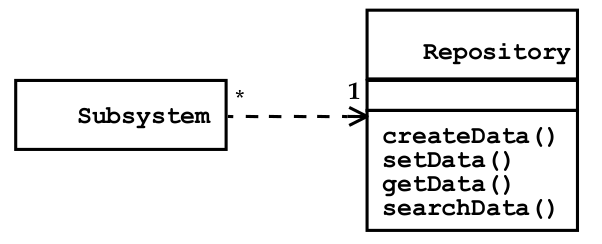
\includegraphics[width=.75\linewidth]{images/pattern_repository.png}
\newpage

\subsection{Blackboard Pattern}
Experts throwing knowledge onto a blackboard (repository) which might be correct or not. Some can be extracted to higher order knowledge and other might be rejected.\\
Structure:\\
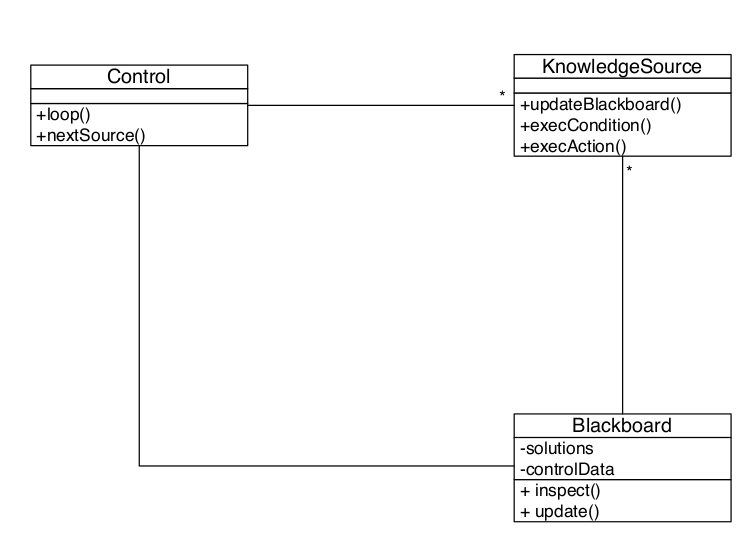
\includegraphics[width=\linewidth]{images/pattern_blackboard.png}
The knowledge sources inspect the current content of the blackboard and create new hypotheses.
Control handles the control flow of the knowledge sources.\\
The blackboard pattern is used when no algorithm for the problem is known.\\
\\
\textbf{6 Steps to Realize a Blackboard Pattern}
\begin{enumerate}
  \item Define the Problem (Identify the application domain, the requirements and the actors)
  \item Define the solution space (top-level and intermediate)
  \item Identify the knowledge sources
  \item Define the blackboard (not every information has to be understandable for every knowledge source)
  \item Define control
  \item Implement the knowledge sources (split into condition part and action part, use computational intelligence or conventional methods)
\end{enumerate}
\newpage

\subsection{Client-Dispatcher-Server Pattern}
The client-dispatcher-server pattern decouples the client from the server.
Usually the client had to know where the server is, now the server is even dynamically interchangeable (server registers to the dispatcher on startup/runtime) what is good for re-configurations and fault tolerance.\\
\begin{minipage}{.5\textwidth}
  Structure:\\
  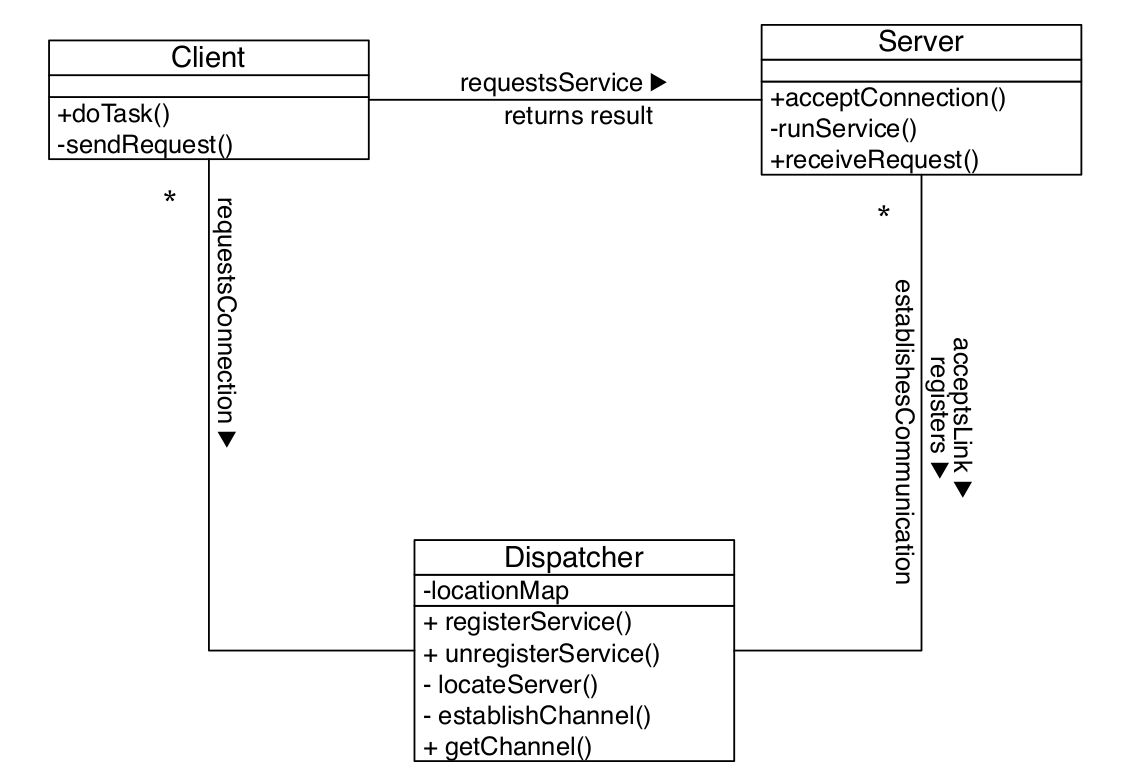
\includegraphics[width=\linewidth]{images/pattern_client_dispatcher_server.png}\\
\end{minipage}
\begin{minipage}{.5\textwidth}
  \vspace{1em}
  Eventflow:\\
  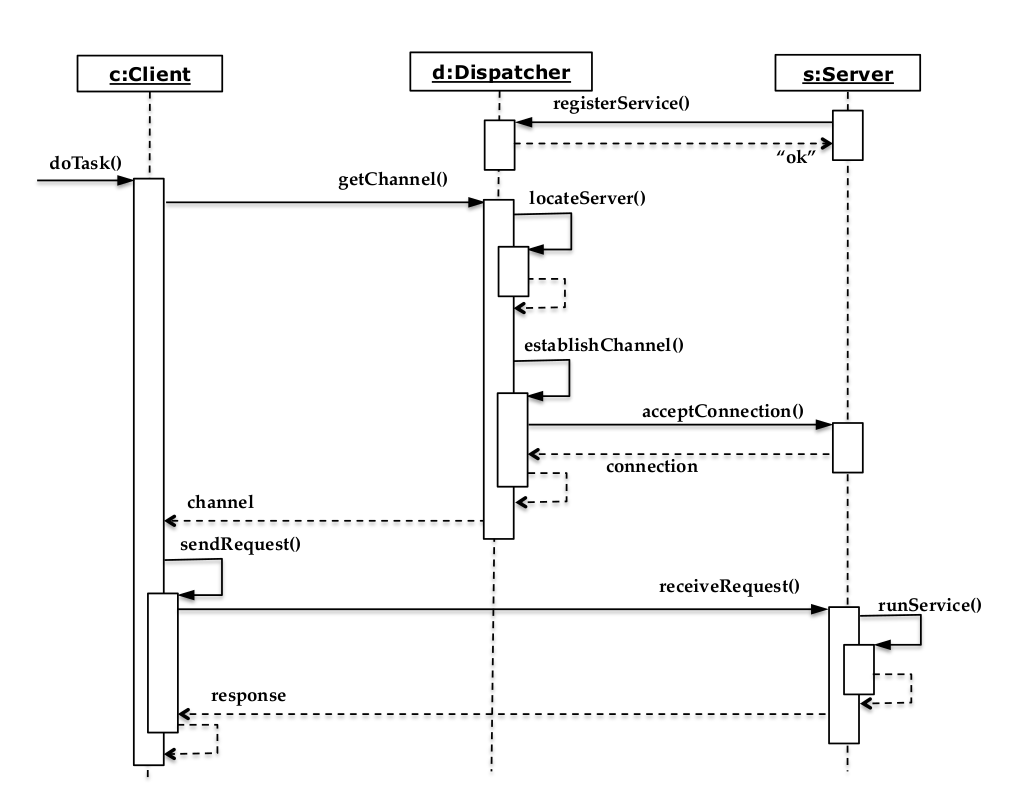
\includegraphics[width=\linewidth]{images/eventflow_client_dispatcher_server.png}
\end{minipage}\\
\\
\textbf{Communication Protocols:}
\begin{description}
  \item[CDprotocol:] Specifies how to ask for servers and handles communication errors.
  \item[DSprotocol:] Specifies how the server registers with the dispatcher and determines the step necessary for a client to establish a connection.
  \item[CSprotocol:] Specifies the communication between client and server.
\end{description}

\textbf{6 Steps to Implement Client-Dispatcher-Server}
\begin{enumerate}
  \item During system design identify the subsystems that act as clients and servers
  \item Decide on the communication mechanism to be used for the protocols (Shared memory, sockets)
  \item Specify the protocols
  \item Decide on a naming scheme for the dispatcher (URLs are ok, IPs not)
  \item Implement the dispatcher
  \begin{enumerate}
    \item Decide how to implement the 3 protocols (sockets, RPM)
    \item Implement requests, responses and errors
    \item Implement a repository that maps server names to addresses
  \end{enumerate}
  \item Implement the client and server (also: when does the server register? Startup or runtime?)
\end{enumerate}
\newpage

\subsection{Broker Pattern}
The broker pattern coordinates the communication between heterogeneous nodes.\\
\\
\textbf{Nonfunctional Requirements:}\\
\vspace{-1.5em}
\begin{description}
  \item[Low Coupling:] Decoupling of service and communication
  \item[Location Transparency:] Services are independent of the server location
  \item[Runtime Extensibility:] Ability to add, remove, exchange components at runtime
  \item[Platform Transparency:] Clients and servers can be written in different languages.
\end{description}
Structure:\\
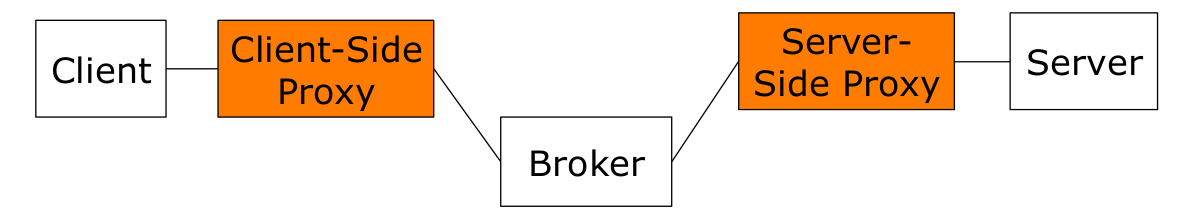
\includegraphics[width=\linewidth]{images/pattern_broker.png}
\textbf{Client-Side Proxy:} Lets the remote object appear as local one, hides the inter-process communication details used for message transfer between client and broker and provides (un-)marshalling/(de-)serialization of parameters and results.\\
\textbf{Server-Side Proxy:} Same as Client-Side proxy only for the server.\\
Eventflow:\\
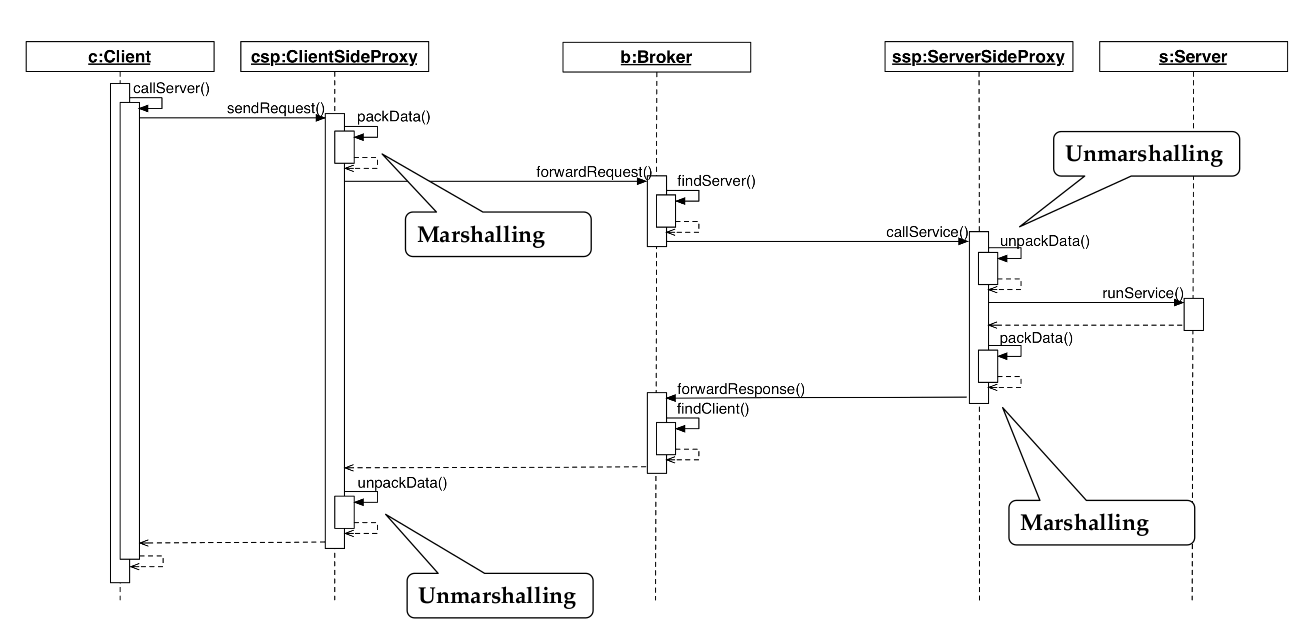
\includegraphics[width=\linewidth]{images/eventflow_broker.png}
\textbf{Steps to Realize a Broker Pattern:}
\begin{enumerate}
  \item Provide the object model and service definitions.
  \item Define the broker service.
  \item Implement the broker component and proxy object at the client and server side.
  \item Implement the client and server.
\end{enumerate}


\newpage
